
\section{Visualisierungen}

\subsection{Analyse der Anwendungsaufgaben}

Analysieren sie die konkreten Anwendungsaufgaben, die die Lösung des Zielproblems durch die Anwender:innen bearbeitet werden müssen. 
Welche sinnvollen mentale Modelle helfen den Personen bei der Bearbeitung. 
%Welche Visualisierungen helfen den Personen, die die Software verwenden, sinnvolle mentale Modelle aufzubauen. 
Sind diese mentalen Modelle für sie notwendig, um die Aufgaben lösen zu können? Gehen sie bei ihrer Argumentation von den Anwendungsaufgaben aus und kommen sie dann zu den mentalen Modellen, deren Aufbau durch Visualisierungen unterstützt wird. 
\subsection{Anforderungen an die Visualisierungen}

Bei diesem Visualisierungsprojekt sind klare Anforderungen an die Darstellung von Daten von entscheidender Bedeutung. Um potenziellen Käufern eine hilfreiche Entscheidungsgrundlage zu bieten, sollten die Visualisierungen Aspekte wie Fahrzeugpreise, Kilometerstand, Baujahr, etc. einschließen. Eine intuitive Benutzeroberfläche ist unabdingbar, damit die Interessenten mühelos durch die Vielzahl von Angeboten navigieren können. Die Visualisierungen sollten daher die Möglichkeit bieten, Fahrzeuge anhand verschiedener Parameter zu filtern und zu vergleichen. Ein interaktiver Ansatz mit Filteroptionen und Hover-Funktionen könnte dabei helfen, detaillierte Informationen zu einzelnen Fahrzeugen abzurufen. Die visuelle Darstellung sollte sowohl informativ als auch ansprechend sein, um die Benutzererfahrung zu optimieren und eine effektive Entscheidungsfindung zu ermöglichen.  \\
Basierend auf diesen Metaanforderungen werden konkrete User Stories formuliert, die im Rahmen des Projektes addressiert werden sollen. \\
Funktionale User Stories: \\
\begin{enumerate}

    \item Als Nutzer möchte  Fahrzeuge anhand verschiedener Parameter wie Preis, Kilometerstand und Baujahr zu vergleichen, um schnell einen Überblick über die verfügbaren Optionen zu erhalten.
    
    \item Als Nutzer wünsche ich mir einen benutzerfreundlichen Parallelplot, der alle relevanten Informationen zu einzelnen Fahrzeugen auf einen Blick darstellt. Damit kann ich die Zusammenhänge zwischen den verschiedenen Parametern besser verstehen und gezielt nach meinen Präferenzen filtern.
    
    \item Als Nutzer interessiere ich mich für einen Star Plot, der mir eine visuelle Zusammenfassung der wichtigsten Merkmale verschiedener Fahrzeugmarken bietet. Dadurch kann ich schnell erkennen, wie sich die Marken in Bezug auf verschiedene Parameter unterscheiden.
\end{enumerate}
Nichtfunktionale User Stories: \\
\begin{enumerate}
    \item Als Anwender möchte ich eine ansprechende und intuitive Oberfläche erleben, die meine Navigation durch die Gebrauchtwagenanzeigen erleichtert. Die Visualisierungen sollten informativ und leicht verständlich sein, um mir eine effiziente Entscheidungsfindung zu ermöglichen.
    
    \item Als Nutzer erwarte ich, dass die Visualisierungen eine hohe Benutzerfreundlichkeit bieten, einschließlich interaktiver Elemente wie Filteroptionen und Hover-Funktionen. Dadurch kann ich gezielt nach meinen Anforderungen suchen und zusätzliche Details zu einzelnen Fahrzeugen abrufen.
    
    \item Als Anwender möchte ich die Möglichkeit haben, die Visualisierungen individuell anzupassen, indem ich verschiedene Parameter auswähle oder abwähle. Dadurch kann ich meine Suche und Analyse personalisieren und mich auf die für mich relevanten Informationen konzentrieren.
    
\end{enumerate}

Aus diesen User Stories wurden dann funktionale und nicht funktionale Anforderungen in einem Use-Case Diagramm (Abbildung \ref*{fig:uc_diagram}) erstellt. \\
\begin{figure}
    \centering
    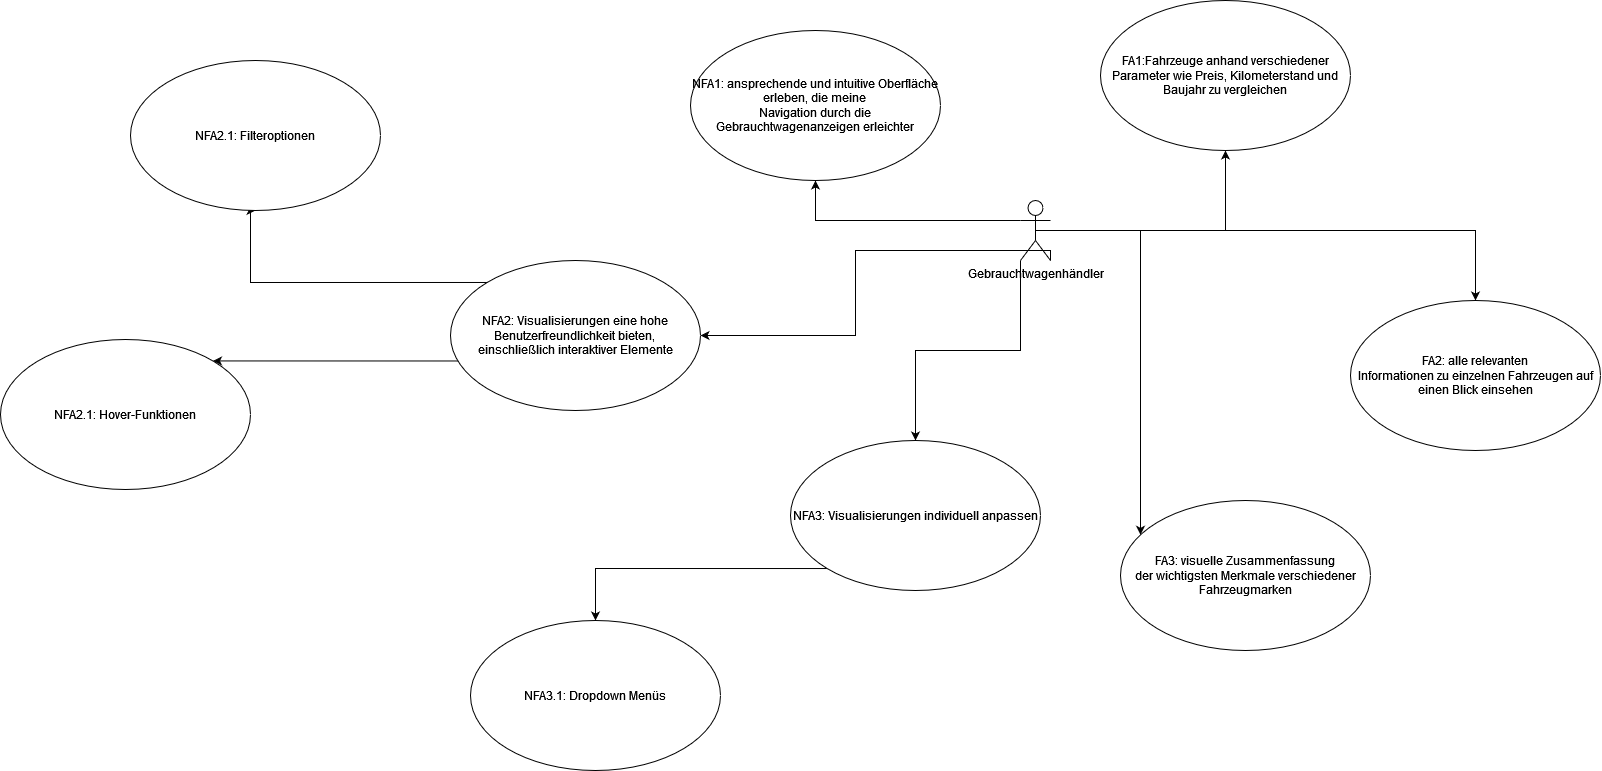
\includegraphics[scale=0,5]{img/uc_diagram.png}
    \label{fig:uc_diagram}
\end{figure}


\subsection{Präsentation der Visualisierungen}
Präsentieren sie die visuelle Abbildungen und Kodierungen der Daten und Interaktionsmöglichkeiten. 
Sie müssen  begründen, warum und wie gut ihre Designentscheidungen die erstellten Anforderungen erfüllen. 
Weiterhin müssen sie begründen, warum die gewählte visuelle Kodierung der Daten für das zulösenden Problem passend ist.
Typische Argumente würden hier auf Wahrnehmungsprinzipien und Theorie über Informationsvisualisierung verweisen. 
Die besten Begründungen diskutieren explizit die konkrete Auswahl der Visualisierungen im Kontext von mehreren verschiedenen Alternativen. 
Machen sie hier nicht den Fehler, einfach nur Visualisierung aus den vorgegebenen Bereichen zu diskutieren, weil das in der Regel nicht sinnvoll ist.
Wenn sie sich für einen Scatterplot entschieden haben, ist ein Zeitreihendiagramm in der Regel keine Alternative.
Diskutieren sie also nicht einfach Zeitreihendiagramme, weil sie in den Anforderungenen an das Projekt neben Scatterplots stehen, sondern suchen sie nach echten alternativen Visualisierungen, die zum Aufbau eines vergleichbaren mentalen Modells führen. 
Diskutieren sie die Expressivität und die Effektivität der einzelnen Visualisierungen. 

Die eben beschriebenen Präsentationen und Begründungen sollen für jede der drei folgenden Visualisierungen durchgeführt werden. 
\subsubsection{Visualisierung Eins}
\subsubsection{Visualisierung Zwei}
\subsubsection{Visualisierung Drei}

\subsection{Interaktion}
Die präsentierten Visualisierungstechniken müssen interaktiv zu einer Anwendung verknüpft werden.
Die Interaktion mit einer Visualisierung soll in den anderen Visualisierungen zu einer Änderung führen. 
Erklären sie die möglichen Interaktionen mit den einzelnen Visualisierungen und die möglichen Verknüpfungen zwischen ihnen. Begründen Sie warum die konkreten Interaktionen umgesetzt wurden und welche Zwecke für die Anwenderinnen mit ihnen unterstützt werden. Begründen sie ebenfalls warum sie andere Interaktionsmöglichkeiten nicht umgesetzt haben. Wenn sie keine der geforderten Interaktionen umsetzen, erhalten Sie im gesamten Projekt deutlichen Punktabzug. 
